\chapter{Evaluation}

Dieses Kapitel beschreibt die finale Evaluation der HoloLens Planner App mit Handwerkern. Zu erst wird die Durchführung erklärt und anschließend die gewonnenen Erkenntnisse aus Fragebogen und den nachfolgenden Gesprächen. Dabei wird genauer darauf eingegangen, wie gebrauchstauglich die Applikation den Handwerkern erscheint, wie sie die Belastung bei ihrer Benutzung einschätzen, ob sie die Technologie Augmented Reality zur Unterstützung ihrer Arbeit in Zukunft akzeptieren würden, wie sie die Erfahrung mit der Applikation fanden und wie man diese noch entwickeln könnte. Es wurden sieben verwertbare Fragebögen und zehn Interviews erzeugt.

\section{Durchführung der Evaluation}

Die Tests wurden bei zehn Handwerkern einzeln, an unterschiedlichen Tagen, zu Hause mit der Microsoft HoloLens und der HoloLens Planner Applikation durchgeführt. Zur Ausführung der Tests wurde den Handwerkern anfangs grob der Umfang dieser Masterarbeit erklärt und was damit bezweckt wird. Anfangs wurde durch Literaturrecherche der aktuelle Stand der Digitalisierung in Handwerksbetrieben und KMUs festgestellt. Um die Materie der Arbeit auf dem Bau kennenzulernen und im Beruf eines Handwerkers Erfahrungen zu machen, die vorher nicht bestanden, wurde eine Ethnographie zum Handwerk des Fliesenlegers durchgeführt. Dadurch wurden Ansatzpunkte für die Unterstützung durch Technologie, genauer durch die Nutzung von Augmented Reality, für Fliesenleger gefunden. Aus diesen Funden wurde eine AR Applikation für die Microsoft HoloLens entwickelt, welche Handwerker beim Kundengespräch, durch virtuelles Fliesenverlegen, sowie beim Fliesen verlegen, durch einblenden eines blauen Rasters helfen soll. Diese Applikation gilt es nun mit Handwerkern zu testen und ihre Meinung darüber zu erheben. 

Die Daten wurden in 3 Phasen erhoben. 

\begin{itemize}
	\item Testen der Applikation in einem vordefinierten Szenario
	\item Ausfüllen des Fragebogens
	\item Unstrukturiertes Gespräch
\end{itemize}

Zum Testen wurde jeweils eine große, freie Fläche benötigt. Den Probanden wurde das Szenario erst erklärt und anschließend wurden sie durch die Applikation geleitet. Es ging darum einen viereckigen Boden im Raum zu markieren und Fliesen darauf zu verlegen, den Verlegeassistenten zu aktivieren und Daten über die Fläche auszulesen. Erst platzierte jeder Proband vier Eckpunkte im Raum. Diese mussten nicht zwingend in tatsächlichen Ecken platziert werden, da das teilweise aus Platzgründen auch nicht möglich war. Nachdem die Fläche so markiert wurde, wählte sie eine Fliese aus, die sie verlegen wollten. Breite und Länge dieser konnten sie beliebig modifizieren. Anschließend legten sie sie auf dem abgesteckten Boden aus. Es wurde ihnen Zeit gegeben sich im Raum zu bewegen und das Bild aufzunehmen. Anschließend aktivierten sie den Verlegeassistenten, welcher nur die Fugen in blau auf dem Boden anzeigt. Wieder hatten sie Zeit, um sich mit dem Feature auseinander zu setzen. Zuletzt öffneten sie erneut das Bodenmenü und bekamen die Daten Fläche, Umfang und Anzahl der Fliesen angezeigt. Damit war der Test beendet.

Von da ging es direkt, ohne viel Kommunikation zum Fragebogen über, den sie freiwillig ausfüllen sollten. Dabei wurde ihnen nur kurz erklärt, wie dieser auszufüllen war. Unterstützt wurden sie dabei nur, wenn ihnen ein Wort undeutlich war. Ansonsten wurde dabei nicht geredet und sie füllten den Fragebogen selbstständig aus.

Zum Abschluss wurde ein unstrukturiertes Gespräch mit jedem Probanden geführt. Dabei sollten diese einfach über ihre Gedanken zu dem Experiment sprechen. Falls das Gespräch stagnierte wurde es mit Fragen, wie zum Beispiel \enquote{Was fanden Sie gut an der Applikation}, \enquote{Welche Funktionalitäten würden Sie sich noch wünschen} oder \enquote{Was hat Ihnen an der Applikation nicht gefallen} wieder angekurbelt. Generell waren die Handwerker jedoch gut im Redefluss und brachten viele eigene Ideen ein und dachten die bisherige Idee weiter. Diese Gespräche wurden, nach Absprache mit den Probanden, teilweise aufgezeichnet. Während jeder Unterhaltung wurden Notizen angefertigt, welche die Aussagen der Handwerker indirekt festhielten.

\section{Ergebnisse des Fragebogens}

Diese Sektion zeigt die Ergebnisse der, durch die Handwerker, ausgefüllten Fragebögen. Alle Daten die hier aufgezeigt werden beziehen sich auf die sieben verwertbaren Fragebögen, die korrekt ausgefüllt wurden. 

\begin{figure}[h]
	\begin{center}
		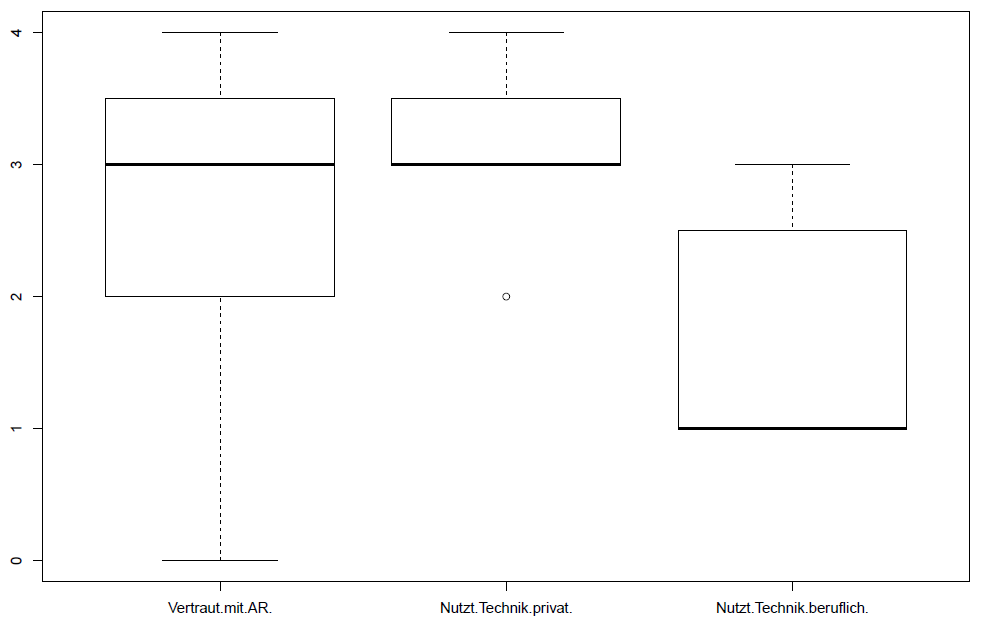
\includegraphics[scale=0.5]{Resources/Evaluation/allgemein.png}
		\label{allgemein}
		\caption{Erhobene allgemeine Daten}	
	\end{center}
\end{figure}

Alle Probanden waren männlich und zwischen 21 - 54 Jahre, fünf davon unter 40 Jahre und zwei über 40 Jahre, alt. Durchschnittlich gaben sie an mit der Technologie Augmented Reality gut vertraut zu sein. Das könnte auf die weite Verbreitung von VR in den letzten Jahren zurückzuführen sein und darauf, dass man diese Technologien häufig auf Messen oder sogar in Museen ausprobieren kann. Allerdings reichen die Angaben von nicht bis sehr vertraut. Im privaten Umfeld nutzen die Handwerker häufig technologische Hilfsmittel, im beruflichen hingegen eher weniger häufig. Das könnte ein weiteres Indiz sein, dass die Digitalisierung im Handwerk noch nicht weit fortgeschritten ist.

Privat nutzt jeder Handwerker mindestens Computer und Smartphone. Über die Hälfte der Probanden gaben an auch von Tablets und teilweise Smartwatches Gebrauch zu machen. Das kann darauf hindeuten, dass sie technisch versiert sind und erklärt auch, warum sie die Nutzung der Microsoft HoloLens schnell, nach einmaligem Erklären, verstanden und umsetzen konnten. \\
Beruflich nutzen über die Hälfte der Handwerker Computer und Smartphone. Einzelne Probanden gaben an nur den Computer oder nur eine Smartphone zu nutzen. Knapp die Hälfte der Probanden setzen auch Tablets in ihrem Beruf ein und einer davon auch eine Smartwatch. Interessant ist, dass zwei der Handwerker Laser zum vermessen nutzen. Laut ihren Aussagen ermöglichen diese ihnen die Messungen noch genauer vorzunehmen, Messfehlern vorzubeugen und so auch besonders kleine Fugen von unter 3mm präzise und konsistent legen zu können. Das nur zwei der sieben Handwerker Laser verwenden kann darauf hindeuten, dass noch kein Großteil der Handwerker alle Möglichkeiten an technischen Hilfsmitteln, welche momentan verfügbar sind, zu ihrem Vorteil nutzen.

Die nächsten Abschnitte zeigen die Auswertung der psychologisch getesteten Fragen aus \ref{fragebogen}. Aussagen der Handwerker aus den Interviews fließen dabei mit ein und helfen die Ergebnisse zu interpretieren.

\subsection{Gebrauchstauglichkeit}

Mit Hilfe der SUS wird bestimmt, wie Gebrauchstauglich und Benutzerfreundlich die Handwerker den HoloLens Planner fanden. \\
Der Durchschnittswert aller SUS Wertungen beträgt 85\% (siehe Abbildung \ref{sus_allBox}). Laut \cite{TODO:WebsitevonKai} bedeutet das für die Applikation eine gute bis exzellente Usability. Insgesamt konnten die Handwerker die Applikation also gut bedienen und empfanden diese als nicht zu kompliziert, was dafür sprechen kann, sie auch in ihren Arbeitsalltag zu integrieren. Wie Krcmar \cite{hateful_six_krcmar} schon feststellte, ist eine einfache Bedienung und Gebrauchstauglichkeit ein entscheidender Faktor, ob eine neue Technologie akzeptiert wird oder nicht. Dieses Ergebnis deutet positiv in diese Richtung. \\
Alle Probanden bis auf zwei werteten die Usability des HoloLens Planners vergleichsweise hoch, das heißt mit einem Wert von 80 oder mehr (siehe Abbildung \ref{sus_all}). Dabei handelt es sich um die Probanden unter 30 Jahren. Diese sind mit mehr technischen Medien aufgewachsen und könnten daher einen besseren Zugang zu neuen Technologien, wie Augmented Reality haben. Die beiden Ausreißer, SUS-Wert 72,5 und 65, stammen von den Probanden über 40. Es wurde bereits erwartet, dass für diese die Bedienung der Microsoft HoloLens und der Applikation schwerer ist. Die Daten deuten darauf hin, dass diese Vermutung stimmt. Allerdings kann man bei einer kleinen Versuchsmenge von sieben Personen nicht genau sagen, ob das der Fall ist. 

\begin{figure}[h]
	\begin{center}
		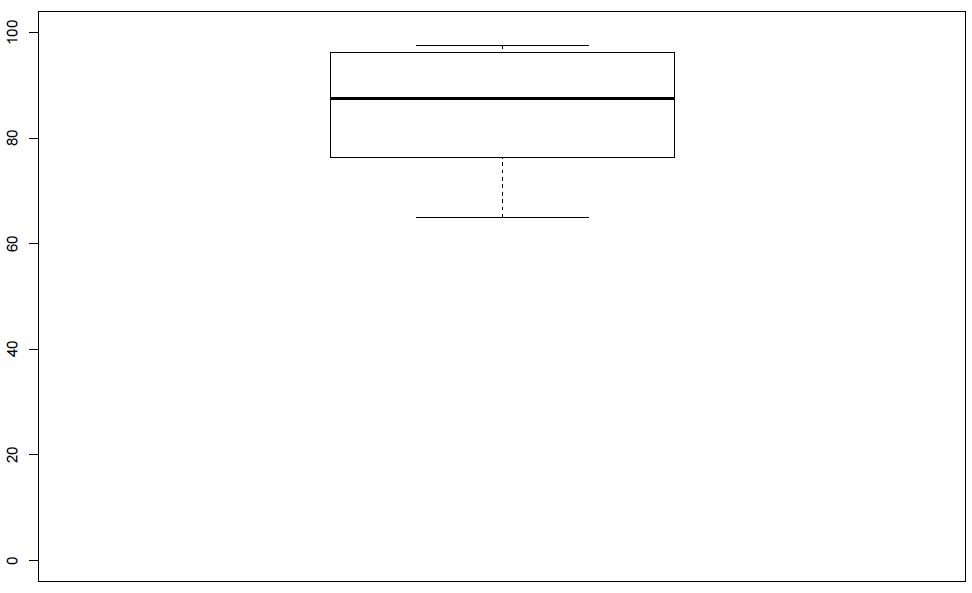
\includegraphics[scale=0.5]{Resources/Evaluation/sus_totalBox.png}
		\label{sus_allBox}
		\caption{Verteilung der SUS-Werte}	
	\end{center}
\end{figure}

\begin{figure}[h]
	\begin{center}
		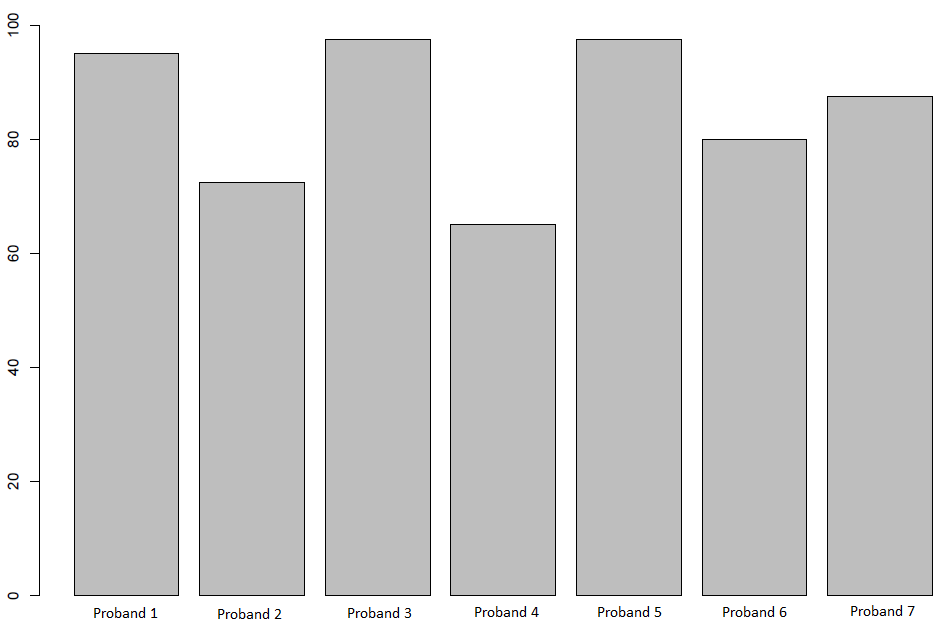
\includegraphics[scale=0.5]{Resources/Evaluation/sus_allTotals.png}
		\label{sus_all}
		\caption{SUS der einzelnen Probanden}	
	\end{center}
\end{figure}

\begin{figure}[H]
	\begin{center}
		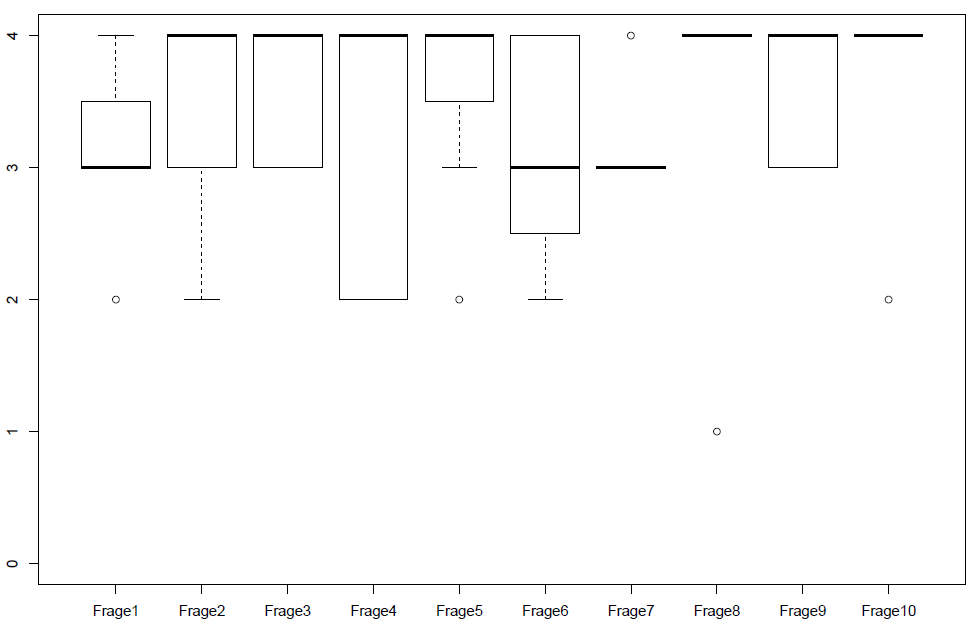
\includegraphics[scale=0.5]{Resources/Evaluation/sus_allQuestionsBox.png}
		\label{sus_questionsBox}
		\caption{Verteilungen der Antworten auf die einzelnen Fragen der SUS}	
	\end{center}
\end{figure}

In Abbildung \ref{sus_questionsBox} fallen Besonderheiten bei den Fragen 5, 8 und 10 auf. \\
Bei Frage 5 gaben alle Probanden bis auf zwei volle Punktzahl. Beide sind über 40 Jahre alt und dadurch wahrscheinlich technisch weniger versiert und äußern ihre Meinung kritischer. Die Angabe des Probanden, welcher die Frage mit 2 Punkten bewertete, passt zu seinen Aussagen im Interview, wo er angibt, dass das blaue Raster zu ungenau sei und dass es definitiv ein Problem sei, dass es nicht mehr eingeblendet wird, wenn er zu nahe ran gehe. Der andere Proband ist, laut Interview, sehr mit der Applikation zufrieden. Eine Abweichung von einem Punkt hat auch keine große Aussagekraft. \\
Das alle Probanden voll Punktzahl gaben, bis auf Proband 4, der nur einen Punkt gab bei Frage 8, fällt deutlich auf. Dabei ist Interessant, dass der Handwerker im Interview angab, dass er sich mit der App sehr vertraut fühle, die Bedienung jedoch als umständlich empfand. Das könnte allerdings nur auf die Funktionalitäten und Möglichkeiten bezogen sein, nicht auf die Bedienung selbst. Diese könnte ihm schwer fallen, da er zu den älteren Probanden zählt. Der andere Handwerker über 40 wiederum gab volle Punktzahl. Er verwendet jedoch bei der Arbeit auch Laser und könnte daher mit technischen Neuerungen besser zurecht kommen. \\
Bei Frage 10 gaben auch alle Probanden bis auf Nummer 4 volle Punktzahl. Hier ist die Vermutung, dass er sich damit auf die Erklärung der Funktionalitäten vor dem Test bezog und auf die Eingewöhnungsphase. Proband 2, welcher auch über 40 Jahre alt ist und angab nicht mit AR vertraut zu sein gab hier wiederum volle Punktzahl. Daraus lässt sich also leider kein guter Schluss ableiten.

\subsection{Arbeitsbelastung}

Mithilfe des NASA-TLX wurde die empfundene Arbeitsbelastung der Handwerker beim Nutzen der HoloLens Planner Applikation gemessen. Mit einem Durchschnittswert von ca. 25 von 100 ist die Belastung eher gering einzuschätzen (siehe Abbildung \ref{nasa_all}). Da AR eine relativ neue und unbekannte Technologie ist, wurde erwartet, dass dieser Wert durchaus höher ist. Interessant ist dabei, dass die Probanden 2 und 4, die über 40 Jährigen, Belastungswerte über 30 angaben. Damit lässt sich aber keine auf das Alter bezogene Aussage machen, da Probanden 1, 5 und 6 auch höhere Werte über 25 aufweisen (siehe Abbildung \ref{nasa_allWorkloads}). Proband 7, einer der jüngsten der relativ wenig Technologie in der Arbeit nutzt, kam auf einen Wert unter 10 und damit auf den niedrigsten. Insgesamt lässt sich damit jedoch sagen, dass die Nutzung der Applikation und AR für die Handwerker wenig anstrengend seien könnte, was positiv für den weiteren Einsatz von AR ist. Da hier mit dem ungewichteten NASA-TLX gearbeitet wurde, muss mehr ins Detail gegangen werden, um bessere Aussagen treffen zu können.

\begin{figure}[h]
	\begin{center}
		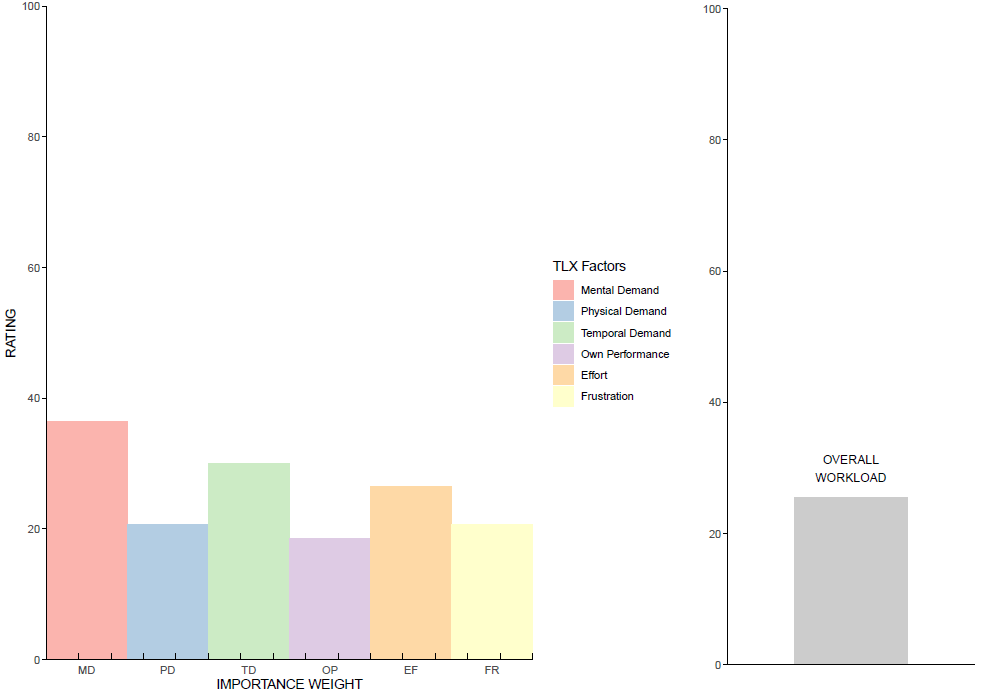
\includegraphics[scale=0.5]{Resources/Evaluation/nasa_all.png}
		\label{nasa_all}
		\caption{Mittelwerte aller Antworten und der Arbeitsbelastung}	
	\end{center}
\end{figure}

\begin{figure}[h]
	\begin{center}
		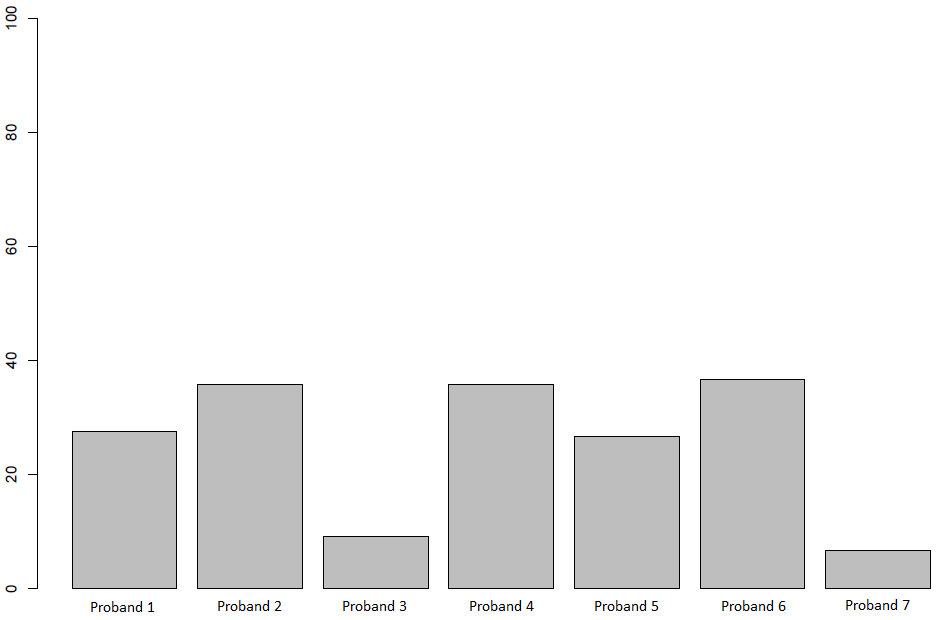
\includegraphics[scale=0.5]{Resources/Evaluation/nasa_allWorkloads.png}
		\label{nasa_allWorkloads}
		\caption{Verteilung aller Ergebnisse für Arbeitsbelastung}	
	\end{center}
\end{figure}

Die Geistige Anforderung fiel mit einem Durchschnittswert von 36 am höchsten aus. AR könnte also mental fordernd seien und den Arbeitern bei der Nutzung auf dem Bau so viel Aufmerksamkeit abverlangen, welche sie dann nicht mehr auf ihre Umgebung richten können. Proband 1 gab dazu an, dass man stark in die Erfahrung mit der Datenbrille eintaucht und so nicht mehr genau wahrnimmt, was um einen herum passiert. Die HoloLens blendet das Umfeld jedoch nicht aus, wie eine VR Brille, weshalb man dieses Phänomen weiter untersuchen sollte. Proband 5 gab an, dass die Applikation das Ausmessen vereinfachen würde, jedoch stimme die Perspektive nicht immer ganz, wodurch man Umdenken muss. Das könnte seine hoch empfundene mentale Belastung erklären. Die Brille sei noch zu unpraktisch und lenke dadurch von der Tätigkeit ab, war die Aussage von Proband 6.

Die Werte für körperliche Anforderung bleiben unter 50, sind gut verteilt und weisen einen Mittelwert von 20 auf. Dadurch lässt sich schließen, dass das Nutzen von AR mental deutlich anspruchsvoller sein könnte als physikalisch. Dies war jedoch anzunehmen. Proband 4 ist hier der einzige Ausreißer mit einem Wert von 45. Dies könnte jedoch auf sein Alter zurückzuführen sein, da er angab, die Verwendung der Applikation fühle sich vertraut an.

Es wurde angenommen, dass die Applikation den Zeitaufwand deutlich verringert. Jedoch empfanden die Handwerker die aufgebrachte Zeit für das Testszenario als nicht gering mit den meisten Werten im Bereich zwischen 30 und 50. Insgesamt stellt diese Dimension mit einem Durchschnittswert von 30 die zweitgrößte Belastung dar. Dies ist eventuell auf das Erstmalige verwenden einer neuen Technologie zurückzuführen. Die Probanden 3 und 7 empfanden den Zeitaufwand jedoch als sehr gering und bestätigten im Interview auch, dass sich mit der Applikation Zeit sparen ließe. Dies müsste in wiederholten Tests geprüft werden.

Mit der Erbrachten Leistung waren alle Handwerker zufrieden, was der Durchschnittswert von 19 bestätigt. Das gleicht sich mit den Aussagen, dass alle sich vorstellen könnten, dass die Technologie Vorteile bringt, ab. Es lässt sich also vermuten, dass die Arbeitsleistung damit verbessert oder zumindest unterstützt werden könnte. Alle Werte sind gut verteilt zwischen 0 und 35. Proband 2, welcher die Wertung 35 abgab, war von dem blauen Raster zur Verlegeunterstützung nicht überzeugt, wodurch sich dieser Wert erklären ließe.

Die Probanden empfanden die Erfahrung mit der Applikation und der Datenbrille als mäßig anstrengend, was der Mittelwert von 26 zeigt. Die Probanden 2 und 4 bewerteten es als anstrengend mit einem Wert über 40. Für sie schien die Nutzung aber generell anstrengender zu sein als für andere Probanden. Handwerker 1 empfand es auch als anstrengend, was sich mit seiner Aussage, dass er sich stark auf die Brille und die Arbeit damit konzentrieren müsse, abgleicht. Interessant sind die Aussagen von Proband 3 und 6, welche sehr gering ausfielen. Sie gaben auch an, das die Applikation leicht zu bedienen sei und ihre Arbeit erleichtern würde.

Die Frustration mit der Applikation hielt sich in Grenzen bei einem Durchschnittswert von 20. Nur Proband 6, mit einem ungewöhnlich hohen Wert von 80 stach hervor. Die Angabe scheint hoch, dafür dass er die Bedienung relativ einfach fand und sich vorstellen konnte, dass die App seine Arbeit erleichtert. Er hält die Technologie jedoch noch für unpraktisch und nicht alltagstauglich, was den hohen Wert erklären könnte. 

\begin{figure}[h]
	\begin{center}
		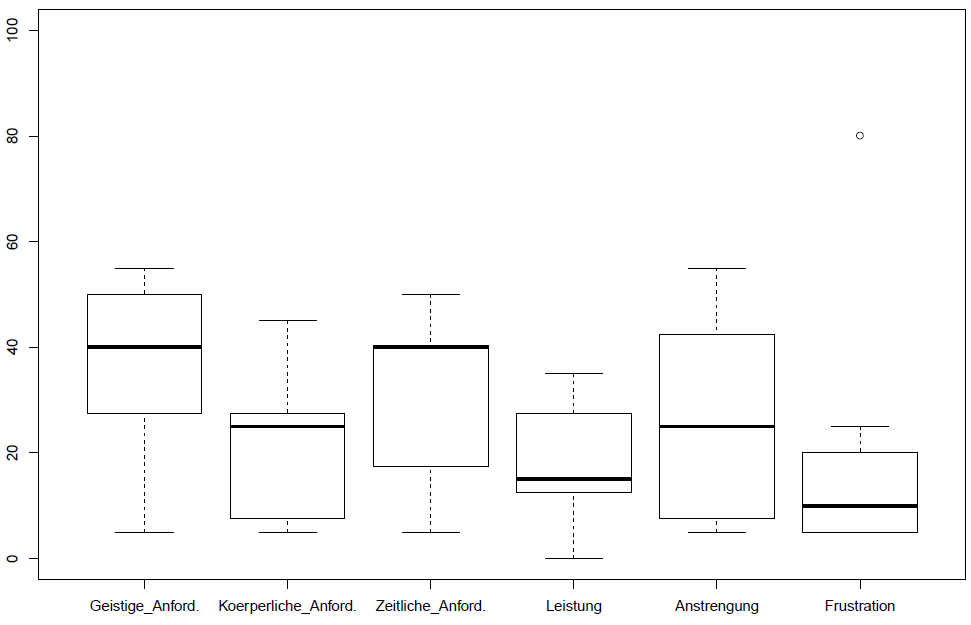
\includegraphics[scale=0.5]{Resources/Evaluation/nasa_questions.png}
		\label{nasa_questions}
		\caption{Verteilung der Antwortwerte der einzelnen Fragen}	
	\end{center}
\end{figure}

\subsection{Akzeptanz der neuen Technologie}

\section{Diskussion der Ergebnisse}

\section{Fazit}